\documentclass[12pt,a4paper,twoside]{article}
\usepackage[colorlinks=true]{hyperref}
\usepackage[utf8]{inputenc}
\usepackage[czech]{babel}
\usepackage{graphicx}
\textwidth 16cm \textheight 25cm
\topmargin -1.3cm 
\oddsidemargin 0cm
\pagestyle{empty}
\begin{document}
\title{Generátor hodin CLKGEN01B}
\author{Jakub Kákona, kaklik@mlab.cz}
\maketitle

\thispagestyle{empty}
\begin{abstract}
Učelem tohoto modulu je poskytnout uživateli dostatečně kvalitní laditelný zdroj frekvenčně stabilního signálu s nízkým šumem vhodného pro konstrukce se špičkovými ADC a obecně v konstrukcích SDR.
\end{abstract}

\begin{figure} [htbp]
\begin{center}
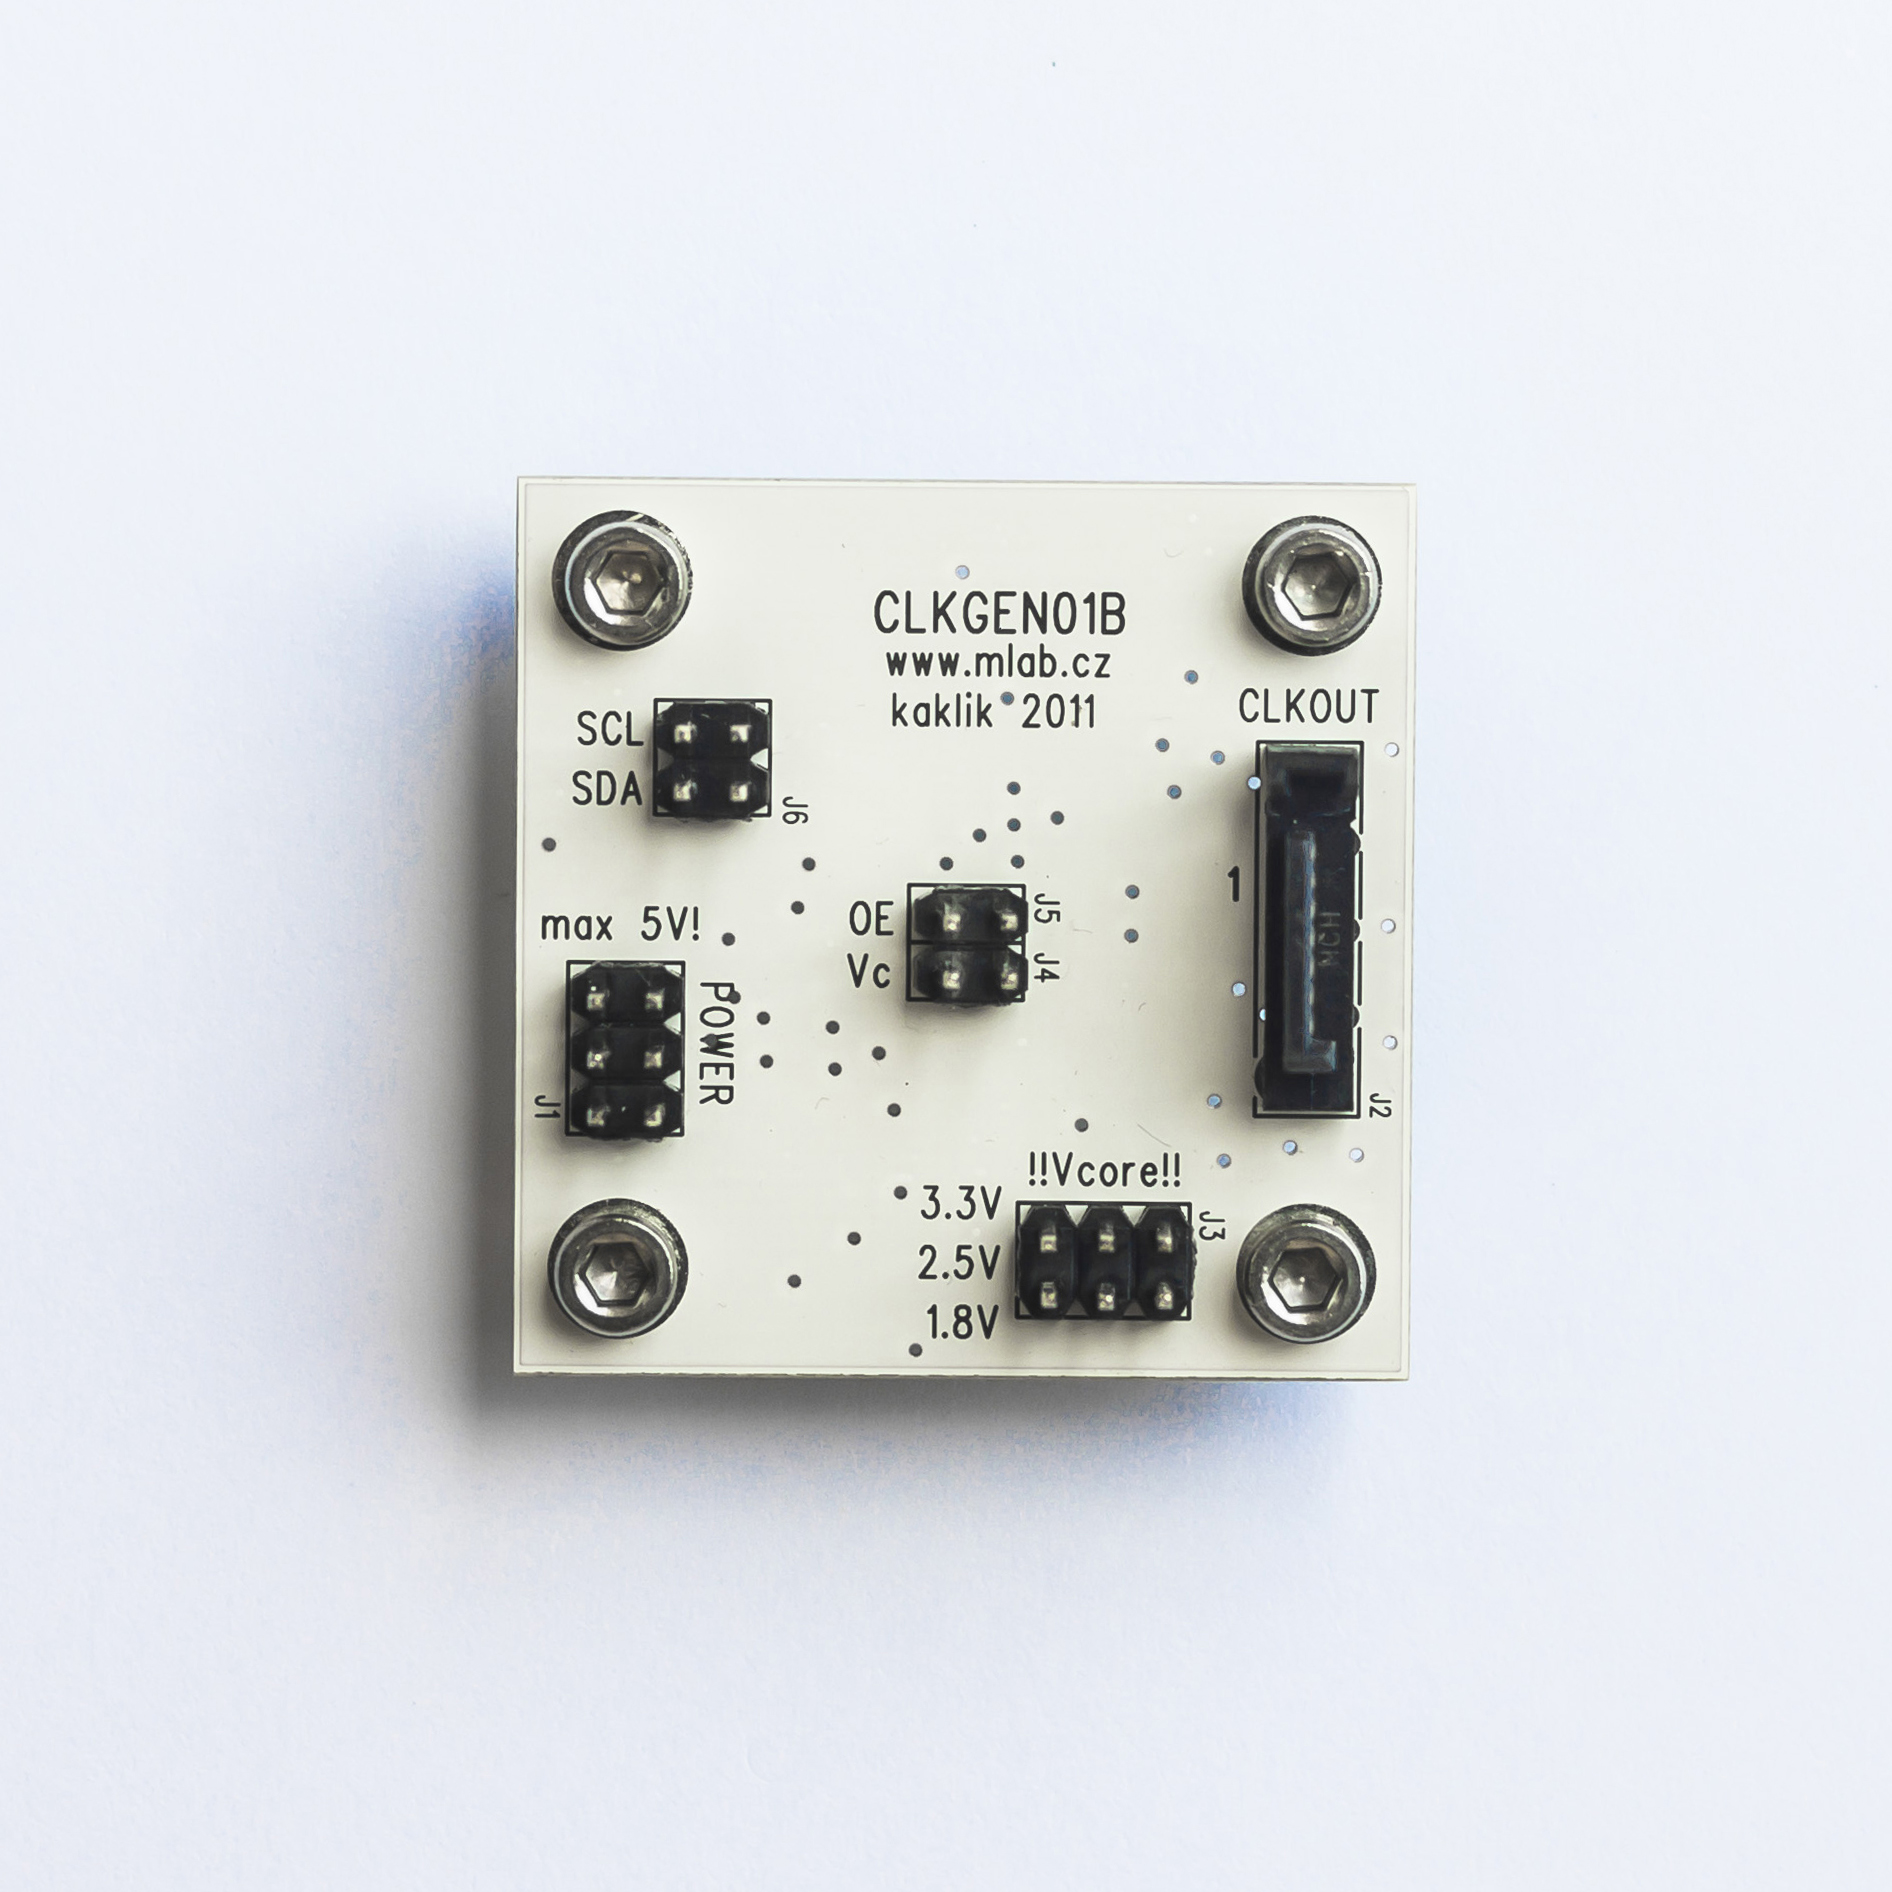
\includegraphics [width=80mm] {CLKGEN01B_Top_Big.jpg} 
\end{center}
\end{figure}

\tableofcontents

\section{Technické parametry}
\begin{table}[htbp]
\begin{center}
\begin{tabular}{|c|c|c|}
\hline
\multicolumn{1}{|c|}{Parametr} & \multicolumn{1}{|c|}{Hodnota} & \multicolumn{1}{|c|}{Poznámka} \\ \hline
Napájecí napětí analogové části & $\pm$10V &  100mA \\ \hline
Napájecí napětí digitální části & +5V &  300mA \\ \hline
Napájecí napětí LNA & do +20V &  max 500mA \\ \hline
Frekvenční rozsah  & 0,5 - 200 MHz & Při osazení vybranými součástkami i 450MHz \\ \hline
IIP3  & $>$ 0dB & Předběžný údaj \\ \hline
Šumové číslo  & $<$ 30dB & \\ \hline
\end{tabular}
\end{center}
\end{table}

\newpage
\section{Popis konstrukce}

\subsection{Zapojení}



\subsection{Odrušení}

\subsection{Mechanická konstrukce}

\section{Výroba a testování}

\subsubsection{Osazení}

\subsubsection{Nastavení}

\section{Programové vybavení}


\begin{thebibliography}{99}
\bibitem{DR2G}{Původní konstrukce } 
\href{http://yu1lm.qrpradio.com/SMT SDR RX DR2G-YU1LM.pdf}{http://yu1lm.qrpradio.com/SMT SDR RX DR2G-YU1LM.pdf}

\end{thebibliography}
\end{document}